\AddToShipoutPicture{\BackgroundPic}

\section*{Jogos Similares}

\begin{enumerate}
	\item {\Large Mark of the Ninja}
	
	Publicado em 2012 pela Klei Entertainment, também é um jogo de plataforma 2D com elementos \emph{stealth}. O jogador controla um ninja e tem a sua disposição itens como explosivos, shurikens, um gancho, e fogos de artifício para destrair os inimigos. Sons causados tanto pelo jogador quanto pelos inimigos são mostrados na tela como círculos. O jogo possui ambientação moderna. 

	\begin{figure}[htb]
		\centering
		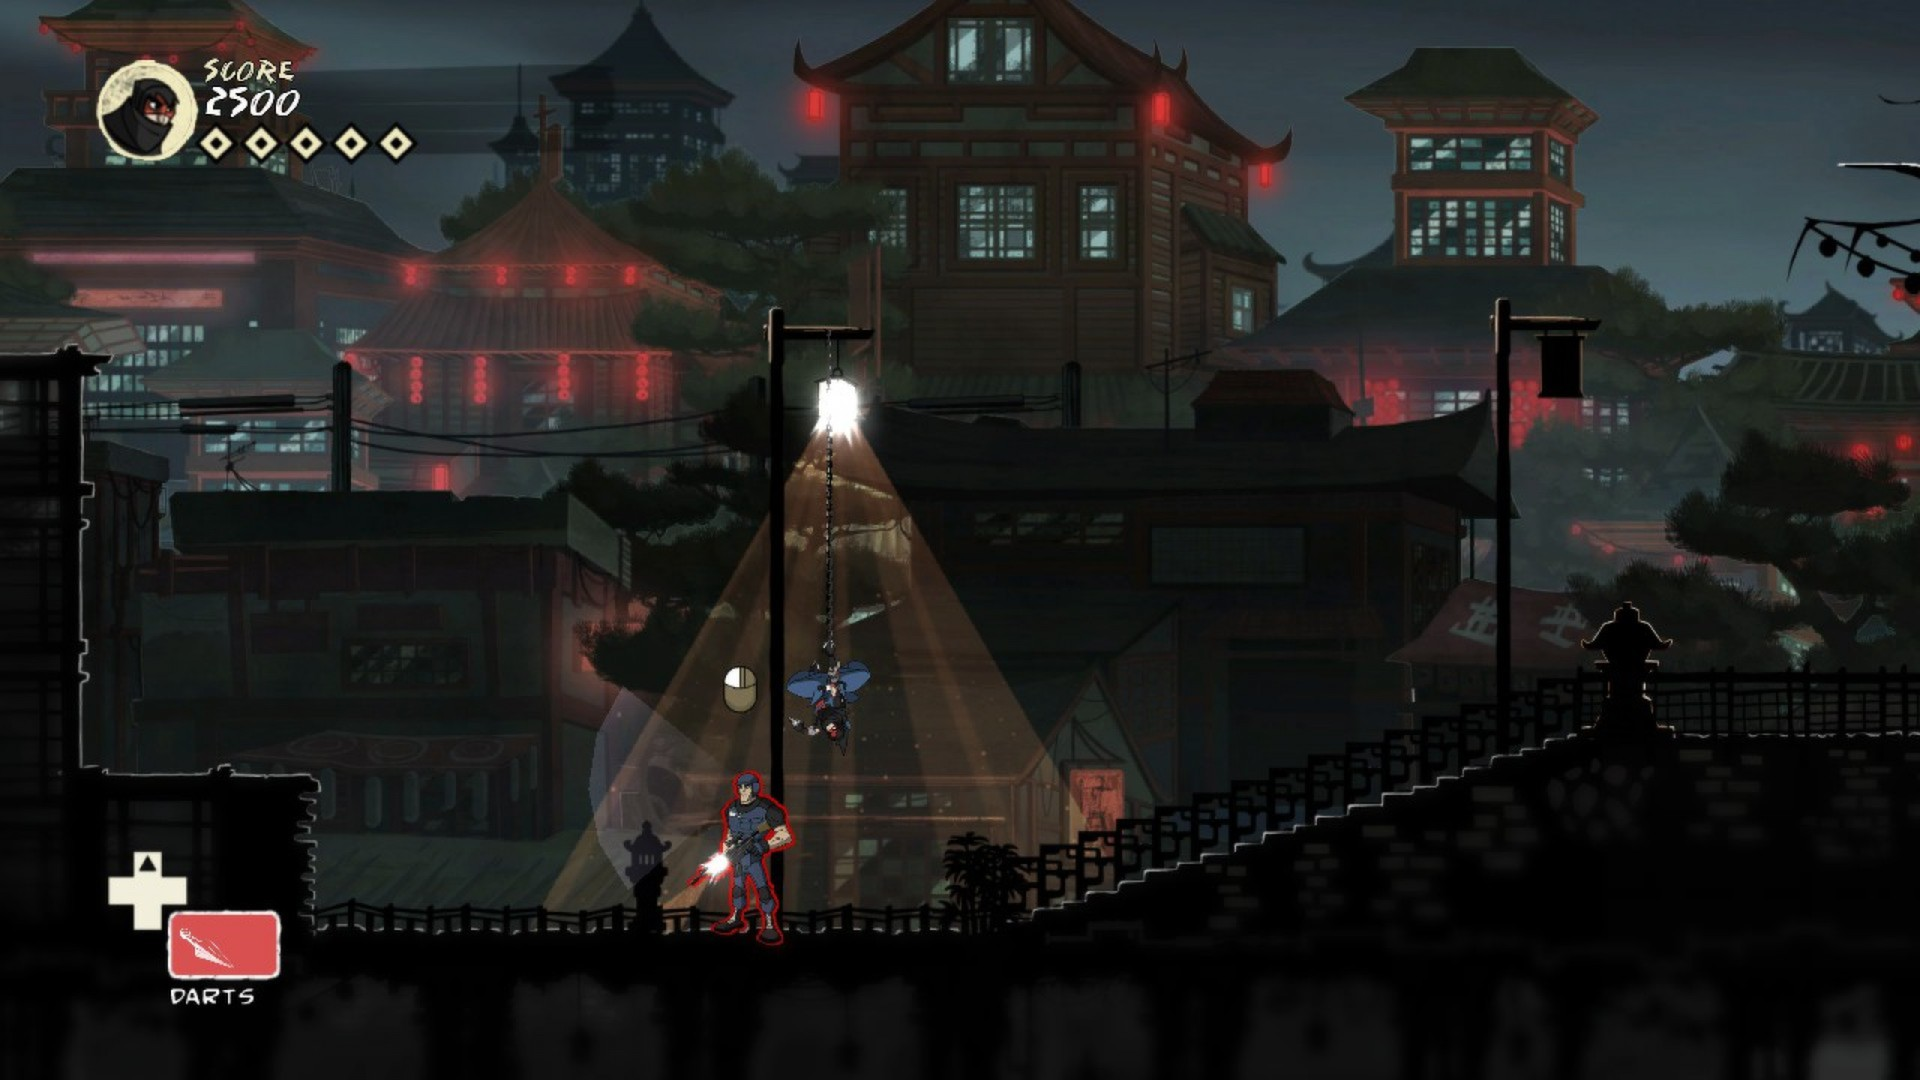
\includegraphics[scale=0.2]{motn}
		\caption{Mark of the Ninja}
	\end{figure}

	\item {\Large Gunpoint}
	
	Publicado em 2013 pelo desenvolvedor independente Tom Francis, Gunpoint não possui muitos elementos tradicionais de plataforma, sendo que maior ênfase é dada a planejamento. A principal mecânica é o chamado Crosslink, que consiste em alterar as conexões elétricas do prédio a ser invadido para abrir caminho (por exemplo, trocar a ligação de um interruptor para que ele abra uma porta ao invés de ligar e desligar uma luz). Essa mecânica também pode ser usada para atacar inimigos (abrir uma porta em cima de um inimigo para desmaiá-lo, por exemplo).

	\begin{figure}[h]
		\centering
		\includegraphics[scale=0.5]{gunpoint}
		\caption{Modo \emph{Crosslink} no jogo Gunpoint}
	\end{figure}

	Dos jogos apresentados, Mark of the Ninja é o mais similar ao jogo proposto, porém Gunpoint oferece uma aproximação diferente para as mecânicas de \emph{stealth}, incluindo elementos \emph{puzzle}. Ambos os jogos foram bem recebidos pela crítica.
	
\end{enumerate}
